\documentclass[aspectratio=169,10pt,xcolor={table,dvipsnames}]{beamer}

% ============================================================
% PACKAGES
% ============================================================
\usepackage[T1]{fontenc}
\usepackage{lmodern}
\usepackage{graphicx}
\usepackage{amsmath,amssymb}
\usepackage{array}
\usepackage{bookmark}
\usepackage{tcolorbox}
\tcbuselibrary{skins}
\usepackage{tikz}
\usetikzlibrary{arrows.meta,positioning,calc,shapes.geometric}

% ============================================================
% MINIMALIST IEEE ACADEMIC PALETTE (Single Navy/Slate Family)
% ============================================================
\definecolor{Navy}{RGB}{11,37,69}           % Primary Deep Navy
\definecolor{SlateBlue}{RGB}{28,64,110}     % Professional Slate Blue Accent
\definecolor{Charcoal}{RGB}{30,41,59}       % High-Contrast Body Text
\definecolor{LightSilver}{RGB}{246,248,251} % Clean Card Background
\definecolor{BorderColor}{RGB}{205,215,226} % Subtle Card Border

\hypersetup{colorlinks=true,linkcolor=Navy,urlcolor=SlateBlue,citecolor=Navy}

% ============================================================
% BEAMER BASE THEME & SETTINGS (Light, Clean, High-Contrast)
% ============================================================
\setbeamercolor{background canvas}{bg=white}
\setbeamercolor{normal text}{fg=Charcoal}
\setbeamercolor{frametitle}{fg=Navy,bg=white}
\setbeamercolor{itemize item}{fg=SlateBlue}
\setbeamercolor{itemize subitem}{fg=SlateBlue}
\setbeamertemplate{navigation symbols}{}
\setbeamertemplate{headline}{}
\setbeamertemplate{itemize item}{\small$\blacktriangleright$}
\setbeamertemplate{itemize subitem}{\scriptsize$\circ$}

% Clean, Minimalist Frametitle (Crisp White Background, Navy Title & Subtle Divider)
\setbeamertemplate{frametitle}{%
  \nointerlineskip
  \begin{beamercolorbox}[wd=\paperwidth,ht=3.0ex,dp=1.0ex,leftskip=0.8cm,rightskip=0.8cm]{frametitle}
    {\fontsize{11}{13}\selectfont\bfseries\color{Navy}\insertframetitle}%
    \hfill{\fontsize{7.5}{9}\selectfont\color{Charcoal!60}\insertframenumber\,/\,\inserttotalframenumber}
  \end{beamercolorbox}%
  \vspace{-2pt}%
  {\color{BorderColor}\hrule height 0.8pt}%
  \vspace{0.14cm}%
}
\setbeamertemplate{footline}{}

% ============================================================
% STANDARDIZED ACADEMIC CARDS (Light Backgrounds, Subtle Borders)
% ============================================================
\tcbset{
  academiccard/.style={
    enhanced,arc=2.5pt,boxrule=0.7pt,
    left=6pt,right=6pt,top=3.5pt,bottom=3.5pt,
    fonttitle=\bfseries\scriptsize,
    colback=LightSilver,colframe=BorderColor,
    coltitle=Navy
  },
  modcard/.style={
    enhanced,arc=2pt,boxrule=0.5pt,
    left=4pt,right=4pt,top=2pt,bottom=2pt,
    fonttitle=\bfseries\fontsize{6.5}{7.5}\selectfont,
    colback=LightSilver,colframe=BorderColor,
    coltitle=Navy
  }
}
\newtcolorbox{navytitlecard}[1]{academiccard,colframe=BorderColor,coltitle=Navy,title={#1}}
\newtcolorbox{plaincard}[1]{academiccard,colframe=BorderColor,coltitle=Navy,title={#1}}

% ============================================================
\begin{document}
% ============================================================

% ------------------------------------------------------------
% SLIDE 1 — TITLE SLIDE (Official Banner + Centered Title + Team)
% ------------------------------------------------------------
\begin{frame}[t,plain]
  % 1. Official College Header Banner (Compact & Proportionally Scaled)
  \vspace*{0.15cm}
  \centerline{
\includegraphics[width=10.8cm,height=1.85cm,keepaspectratio]{college_header.png}}
  \vspace{0.08cm}
  \centerline{\color{BorderColor}\rule{10.8cm}{0.8pt}}

  \vspace{0.22cm}

  % 2. Project Title Box
  \begin{tcolorbox}[
    enhanced,colback=LightSilver,colframe=BorderColor,
    arc=3pt,boxrule=0.8pt,
    left=10pt,right=10pt,top=6pt,bottom=6pt]
    \centering
    {\fontsize{12}{15}\selectfont\bfseries\color{Navy}%
      IT Vault: Skill Mapping, Automated Assessment \&\\[3pt]
      Verified Placement Collaboration Portal}
    \vspace{2pt}\\
    {\fontsize{6.8}{8.2}\selectfont\color{SlateBlue}\bfseries
      Academia-Industry Collaboration \textbullet\ Continuous Skill Analytics \textbullet\ QR Verification}
  \end{tcolorbox}

  \vspace{0.18cm}

  % 3. Team Members (Centered & Professional Academic Layout)
  \begin{columns}[c]
    \begin{column}{0.48\textwidth}
      \begin{tcolorbox}[academiccard,title={Team Member 1}]
        \centering\fontsize{7.5}{9}\selectfont
        \textbf{\color{Navy}Tharunkumar K}\\[2pt]
        {\fontsize{6.5}{7.8}\selectfont\color{Charcoal!80}Reg.\;No:\;\textbf{922524205171}}
      \end{tcolorbox}
    \end{column}

    \begin{column}{0.48\textwidth}
      \begin{tcolorbox}[academiccard,title={Team Member 2}]
        \centering\fontsize{7.5}{9}\selectfont
        \textbf{\color{Navy}Santhoshkumar S}\\[2pt]
        {\fontsize{6.5}{7.8}\selectfont\color{Charcoal!80}Reg.\;No:\;\textbf{922524205148}}
      \end{tcolorbox}
    \end{column}
  \end{columns}

  % 4. Bottom Deployment Status Badge
  \vspace{0.12cm}
  \begin{tcolorbox}[
    enhanced,colback=LightSilver,colframe=BorderColor,
    arc=2pt,boxrule=0.5pt,
    left=4pt,right=4pt,top=2pt,bottom=2pt]
    \centering\fontsize{6.2}{7.5}\selectfont\bfseries\color{Navy}
    Current Status: Active Departmental Pilot Deployment \enspace\textbullet\enspace Pre-Final Year Project (Started 2026)
  \end{tcolorbox}
\end{frame}

% ------------------------------------------------------------
% SLIDE 2 — INTRODUCTION
% ------------------------------------------------------------
\begin{frame}[t]{Introduction}
  \begin{columns}[T]
    \begin{column}{0.485\textwidth}
      \begin{navytitlecard}{1.\;The Placement-Academia Divide}
        \fontsize{6.5}{7.8}\selectfont
        \begin{itemize}\setlength{\itemsep}{1pt}
          \item Traditional college curricula struggle to stay synchronized with rapidly changing industry tech stacks and hiring standards.
          \item Students self-declare skills on paper resumes without standardized, verifiable evidence of practical capability.
        \end{itemize}
      \end{navytitlecard}
      \vspace{0.04cm}
      \begin{plaincard}{2.\;Manual Departmental Workflows}
        \fontsize{6.5}{7.8}\selectfont
        \begin{itemize}\setlength{\itemsep}{0.8pt}
          \item Training \& Placement Officers (TPOs) manage student eligibility, CGPA, and drive registrations via unorganized Google Sheets.
          \item Clerical errors, duplicate applications, and missed company deadlines degrade campus placement efficiency.
        \end{itemize}
      \end{plaincard}
    \end{column}

    \begin{column}{0.485\textwidth}
      \begin{navytitlecard}{3.\;Delayed Skill Deficit Discovery}
        \fontsize{6.5}{7.8}\selectfont
        \begin{itemize}\setlength{\itemsep}{0.8pt}
          \item Students only discover critical competency gaps after getting rejected in final-year campus interview rounds.
          \item Pre-final year students lack automated diagnostic tools to pinpoint and bridge domain deficits early.
        \end{itemize}
      \end{navytitlecard}
      \vspace{0.04cm}
      \begin{plaincard}{4.\;Recruiter Screening Overhead}
        \fontsize{6.5}{7.8}\selectfont
        \begin{itemize}\setlength{\itemsep}{0.8pt}
          \item Corporate recruiters spend over 70\% of initial drive time manually filtering hundreds of unverified candidate profiles.
          \item Lack of authentic practical test logs and mentor reviews creates severe recruitment friction.
        \end{itemize}
      \end{plaincard}
    \end{column}
  \end{columns}

  \vspace{0.04cm}
  \begin{tcolorbox}[
    enhanced,colback=LightSilver,colframe=BorderColor,
    arc=2pt,boxrule=0.6pt,
    left=5pt,right=5pt,top=2pt,bottom=2pt]
    \centering\fontsize{6.3}{7.5}\selectfont
    \textbf{\color{Navy}Core Need:}\;An automated digital portal uniting Students, Faculty/TPOs, and Industry Recruiters through live skill assessments, verified milestone tracking, and tamper-proof QR credentialing.
  \end{tcolorbox}
\end{frame}

% ------------------------------------------------------------
% SLIDE 3 — ABSTRACT: PROBLEM & RESEARCH OBJECTIVE
% ------------------------------------------------------------
\begin{frame}[t]{Abstract\enspace---\enspace Problem \& Objective}
  \begin{tcolorbox}[
    enhanced,colback=LightSilver,colframe=BorderColor,
    arc=2.5pt,boxrule=0.7pt,
    left=8pt,right=8pt,top=4pt,bottom=4pt]
    \fontsize{7.2}{8.8}\selectfont
    \textbf{\color{Navy}Problem Statement (SIH26044):}\quad
    Lack of a unified, verified digital ecosystem for academia-industry collaboration that maps student competencies, streamlines internship/placement drives, and provides objective evidence of practical coding skills.
    \vspace{2pt}
    \begin{itemize}\setlength{\itemsep}{1.5pt}
      \item \textbf{Unverified Claims:}\;Resumes claim multiple languages with zero proof of actual project execution.
      \item \textbf{Fragmented Operations:}\;TPO data scattered across disconnected spreadsheets and forms.
      \item \textbf{Recruiter Distrust:}\;No real-time tamper-proof verification of test scores or academic milestones.
    \end{itemize}
  \end{tcolorbox}

  \vspace{0.08cm}

  \begin{tcolorbox}[
    enhanced,colback=LightSilver,colframe=BorderColor,
    arc=2.5pt,boxrule=0.7pt,
    left=8pt,right=8pt,top=4pt,bottom=4pt]
    \fontsize{7.2}{8.8}\selectfont
    \textbf{\color{Navy}Project Solution \& Objectives (IT Vault):}\quad
    To build, deploy, and validate a full-stack collaboration platform that automates skill verification, placement readiness tracking, and recruiter shortlisting:
    \vspace{2pt}
    \begin{itemize}\setlength{\itemsep}{1.5pt}
      \item \textbf{Target 1:}\;Conduct domain-specific diagnostic assessments with automated competency radar mapping.
      \item \textbf{Target 2:}\;Enable faculty mentors to verify student lab milestones and issue authenticated digital badges.
      \item \textbf{Target 3:}\;Provide QR-authenticated profile transcripts and automated placement drive pipelines.
    \end{itemize}
  \end{tcolorbox}

  \vspace{0.04cm}
  \begin{tcolorbox}[
    enhanced,colback=LightSilver,colframe=BorderColor,
    arc=2pt,boxrule=0.6pt,
    left=6pt,right=6pt,top=2pt,bottom=2pt]
    \centering\fontsize{6.5}{7.8}\selectfont
    \textbf{\color{Navy}Traction:}\;\textbf{Currently deployed as an active pilot in our department}, supporting pre-final year students and faculty coordinators.
  \end{tcolorbox}
\end{frame}

% ------------------------------------------------------------
% SLIDE 4 — ABSTRACT: PROPOSED RESEARCH CYCLE
% ------------------------------------------------------------
\begin{frame}[t]{Abstract\enspace---\enspace End-to-End Operational Cycle}
  \centering
  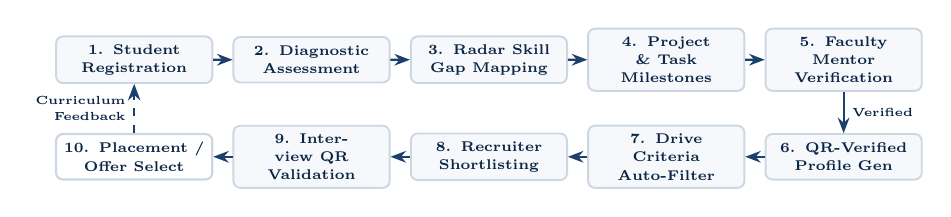
\begin{tikzpicture}[
      scale=0.85,every node/.style={transform shape},
      bNode/.style={draw=BorderColor,fill=LightSilver,rounded corners=2.5pt,
                    minimum width=2.30cm,minimum height=0.68cm,text width=2.10cm,
                    font=\fontsize{6.5}{7.8}\selectfont\bfseries,align=center,text=Navy,line width=0.7pt},
      tNode/.style={draw=BorderColor,fill=LightSilver,rounded corners=2.5pt,
                    minimum width=2.30cm,minimum height=0.68cm,text width=2.10cm,
                    font=\fontsize{6.5}{7.8}\selectfont\bfseries,align=center,text=Navy,line width=0.7pt},
      fNode/.style={draw=BorderColor,fill=white,rounded corners=2.5pt,
                    minimum width=2.30cm,minimum height=0.68cm,text width=2.10cm,
                    font=\fontsize{6.5}{7.8}\selectfont\bfseries,align=center,text=Navy,line width=0.8pt},
      ar/.style={-{Stealth[scale=0.85]},line width=0.8pt,color=SlateBlue}
    ]

    % Row 1: Evidence Ingestion (Left to Right)
    \node(n1)[bNode] at (0, 1.45) {1. Student\\Registration};
    \node(n2)[bNode] at (2.65, 1.45) {2. Diagnostic\\Assessment};
    \node(n3)[bNode] at (5.30, 1.45) {3. Radar Skill\\Gap Mapping};
    \node(n4)[bNode] at (7.95, 1.45) {4. Project \& Task\\Milestones};
    \node(n5)[bNode] at (10.60, 1.45) {5. Faculty Mentor\\Verification};

    % Row 2: Diagnostic & Closed Loop (Right to Left)
    \node(n6)[tNode] at (10.60, 0) {6. QR-Verified\\Profile Gen};
    \node(n7)[tNode] at (7.95, 0) {7. Drive Criteria\\Auto-Filter};
    \node(n8)[tNode] at (5.30, 0) {8. Recruiter\\Shortlisting};
    \node(n9)[tNode] at (2.65, 0) {9. Interview QR\\Validation};
    \node(n10)[fNode] at (0, 0) {10. Placement /\\Offer Select};

    % Phase 1 Arrows
    \draw[ar] (n1) -- (n2);
    \draw[ar] (n2) -- (n3);
    \draw[ar] (n3) -- (n4);
    \draw[ar] (n4) -- (n5);

    % Transition Downward Arrow on Right
    \draw[ar] (n5.south) -- node[right,font=\fontsize{5.5}{6.5}\selectfont\bfseries,color=Navy]{Verified} (n6.north);

    % Phase 2 Arrows
    \draw[ar] (n6) -- (n7);
    \draw[ar] (n7) -- (n8);
    \draw[ar] (n8) -- (n9);
    \draw[ar] (n9) -- (n10);

    % Vertical Closed-Loop Feedback Arrow on Left
    \draw[ar,dashed,line width=0.9pt] (n10.north) -- 
      node[left,font=\fontsize{5.5}{6.5}\selectfont\bfseries,color=Navy,align=right]%
      {Curriculum\\Feedback} (n1.south);
  \end{tikzpicture}

  \vspace{0.12cm}

  \begin{columns}[T]
    \begin{column}{0.485\textwidth}
      \begin{tcolorbox}[academiccard,title={Phase 1 : Assessment \& Milestone Verification (Nodes 1--5)}]
        \fontsize{6.5}{7.8}\selectfont
        Students attempt time-bound domain tests, receive instant skill radar gap scores, and submit project repositories verified by departmental faculty.
      \end{tcolorbox}
    \end{column}
    \begin{column}{0.485\textwidth}
      \begin{tcolorbox}[academiccard,title={Phase 2 : Drive Matching \& QR Validation (Nodes 6--10)}]
        \fontsize{6.5}{7.8}\selectfont
        System auto-screens eligible candidates for posted company drives, enabling recruiters to scan profile QR codes for instant, tamper-proof score verification.
      \end{tcolorbox}
    \end{column}
  \end{columns}

  \vspace{0.08cm}
  \begin{tcolorbox}[
    enhanced,colback=LightSilver,colframe=BorderColor,
    arc=2pt,boxrule=0.6pt,
    left=6pt,right=6pt,top=2.5pt,bottom=2.5pt]
    \centering\fontsize{6.5}{7.8}\selectfont
    \textbf{\color{Navy}Core Novelty:}\;Replaces self-declared claims with an \textbf{end-to-end verified pipeline} combining automated testing, faculty verification, and tamper-proof recruiter validation.
  \end{tcolorbox}
\end{frame}

% ------------------------------------------------------------
% SLIDE 5 — LITERATURE SURVEY (Clean IEEE Monochrome Table)
% ------------------------------------------------------------
\begin{frame}[t]{Literature Survey}
  \vspace{-0.1cm}
  \centering
  {\fontsize{5.8}{7.2}\selectfont
  \renewcommand{\arraystretch}{1.10}
  \begin{tabular}{|c|>{\raggedright\arraybackslash\sloppy}p{4.0cm}|>{\raggedright\arraybackslash\sloppy}p{2.2cm}|c|>{\raggedright\arraybackslash\sloppy}p{4.6cm}|}
    \hline
    \rowcolor{LightSilver}
    \textbf{S.No} & \textbf{Paper Title} & \textbf{Author(s)} & \textbf{Year} & \textbf{Drawbacks \& Research Limitations}\\
    \hline
    \textbf{1} &
    \textbf{Skill Mapping and Competency Verification in Higher Education} &
    Sharma R.\ et al.\ (IEEE Access) & 2024 &
    Theoretical taxonomy mapping only; lacks automated live testing engine and recruiter verification workflow.\\
    \hline
    \rowcolor{LightSilver}
    \textbf{2} &
    \textbf{Automated Placement Portals and Student Filtering Systems} &
    Patel K.\ et al.\ (IEEE TALE) & 2025 &
    Evaluates CGPA-only criteria; ignores practical project repositories and diagnostic coding assessment telemetry.\\
    \hline
    \textbf{3} &
    \textbf{Learning Analytics for Predicting Graduate Employability} &
    Moreno-Marcos P.\ et al.\ (IEEE ICALT) & 2025 &
    Provides predictive metrics but lacks active faculty project verification badges and real-time offline-first lab capability.\\
    \hline
    \rowcolor{LightSilver}
    \textbf{4} &
    \textbf{Outcome-Based Education Frameworks in Engineering Courses} &
    Vargas H.\ et al.\ (IEEE Trans.\ Educ.) & 2024 &
    Defines course outcome matrices; lacks direct industry recruiter portal integration and QR-authenticated PDF generation.\\
    \hline
    \textbf{5} &
    \textbf{Classroom Evaluation of Continuous Assessment Platforms} &
    Jeon J.\ et al.\ (IEEE FIE) & 2026 &
    Confined to isolated lab testing; lacks multi-tier role dashboards for Students, TPOs, and Industry Recruiters.\\
    \hline
  \end{tabular}}

  \vspace{0.10cm}
  \begin{tcolorbox}[
    enhanced,colback=LightSilver,colframe=BorderColor,
    arc=2pt,boxrule=0.7pt,
    left=6pt,right=6pt,top=3pt,bottom=3pt]
    \centering\fontsize{6.5}{7.8}\selectfont
    \textbf{\color{Navy}Identified Research Gap:}\;Existing systems operate in \textbf{fragmented silos} (LMS vs.\ Job Boards vs.\ Coding Sites). No unified solution combines \textbf{diagnostic testing, faculty project validation, TPO batch analytics, and instant recruiter QR verification}.
  \end{tcolorbox}
\end{frame}

% ------------------------------------------------------------
% SLIDE 6 — EXISTING SYSTEM & DRAWBACKS
% ------------------------------------------------------------
\begin{frame}[t]{Existing System\enspace---\enspace Drawbacks}
  \begin{columns}[T]
    % Left Column: Conventional Flowchart
    \begin{column}{0.43\textwidth}
      \begin{navytitlecard}{Conventional Fragmented Flow}
        \centering\vspace{1pt}
        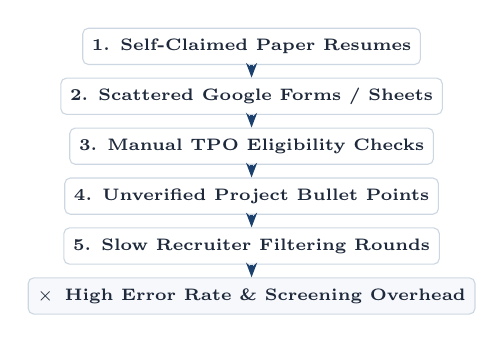
\begin{tikzpicture}[
          node distance=0.16cm,
          bk/.style={draw=BorderColor,fill=white,rounded corners=2pt,
                     minimum width=3.8cm,minimum height=0.46cm,
                     font=\fontsize{6.2}{7.5}\selectfont\bfseries,text=Charcoal},
          ar/.style={-{Stealth[scale=0.8]},thick,SlateBlue}
        ]
          \node(e1)[bk]{1. Self-Claimed Paper Resumes};
          \node(e2)[bk,below=of e1]{2. Scattered Google Forms / Sheets};
          \node(e3)[bk,below=of e2]{3. Manual TPO Eligibility Checks};
          \node(e4)[bk,below=of e3]{4. Unverified Project Bullet Points};
          \node(e5)[bk,below=of e4]{5. Slow Recruiter Filtering Rounds};
          \node(e6)[bk,below=of e5,draw=BorderColor,fill=LightSilver,text=Charcoal]{$\times$\enspace High Error Rate \& Screening Overhead};

          \draw[ar] (e1) -- (e2);
          \draw[ar] (e2) -- (e3);
          \draw[ar] (e3) -- (e4);
          \draw[ar] (e4) -- (e5);
          \draw[ar,SlateBlue,dashed] (e5) -- (e6);
        \end{tikzpicture}
      \end{navytitlecard}
    \end{column}

    % Right Column: Drawbacks
    \begin{column}{0.55\textwidth}
      \begin{plaincard}{Systemic Bottlenecks}
        \fontsize{6.8}{8.2}\selectfont
        \begin{enumerate}\setlength{\itemsep}{2.2pt}
          \item \textbf{Unverified Resumes:}\;Candidates list skills without verified assessment proof.
          \item \textbf{Spreadsheet Chaos:}\;Manual data handling leads to missed deadlines and clerical errors.
          \item \textbf{Recruiter Overhead:}\;Recruiters spend 70\%+ time on preliminary filtering.
          \item \textbf{Late Gap Detection:}\;Students realize skill deficits only after placement rejection.
          \item \textbf{Lab Network Vulnerability:}\;Online portals crash during college network dropouts.
          \item \textbf{No Recruiter Validation:}\;Inability to verify test authenticity during live interviews.
        \end{enumerate}
      \end{plaincard}
    \end{column}
  \end{columns}

  \vspace{0.12cm}
  \begin{tcolorbox}[
    enhanced,colback=LightSilver,colframe=BorderColor,
    arc=2pt,boxrule=0.6pt,
    left=6pt,right=6pt,top=2.5pt,bottom=2.5pt]
    \centering\fontsize{6.5}{7.8}\selectfont
    \textbf{\color{Navy}Critical Consequence:}\;Lack of verified data wastes hundreds of recruiter hours and leaves pre-final year students unprepared for corporate hiring benchmarks.
  \end{tcolorbox}
\end{frame}

% ------------------------------------------------------------
% SLIDE 7 — PROPOSED SYSTEM & ADVANTAGES
% ------------------------------------------------------------
\begin{frame}[t]{Proposed Solution\enspace---\enspace Key Advantages}
  \begin{columns}[T]
    % Left Column: Architecture Overview + Contribution
    \begin{column}{0.46\textwidth}
      \begin{navytitlecard}{IT Vault Integrated Model}
        \fontsize{6.5}{7.6}\selectfont
        \renewcommand{\arraystretch}{1.06}
        \begin{tabular}{@{}cl@{}}
          {\color{Navy}$\blacktriangleright$} & \textbf{Diagnostic Skill Assessments}\\
          {\color{Navy}$+$} & Live Radar Competency Analytics\\
          {\color{Navy}$+$} & Faculty-Verified Project Badges\\
          {\color{Navy}$+$} & Offline-First IndexedDB Persistence\\[1pt]
          \hline\\[-6pt]
          {\color{Navy}$\downarrow$} & \textbf{Automated Placement Drive Filtering}\\
          {\color{Navy}$\downarrow$} & \textbf{Tamper-Proof QR Transcripts}\\
          {\color{Navy}$\downarrow$} & \textbf{TPO Batch-Level Skill Heatmaps}\\
          {\color{Navy}$\downarrow$} & \textbf{Direct Recruiter Shortlisting}\\[1pt]
          \hline\\[-6pt]
          {\color{Navy}$\circlearrowleft$} & \textbf{Continuous Academic-Industry Calibration}
        \end{tabular}
      \end{navytitlecard}
      \vspace{0.04cm}
      \begin{tcolorbox}[
        enhanced,colback=LightSilver,colframe=BorderColor,
        arc=2pt,boxrule=0.6pt,
        left=4pt,right=4pt,top=2pt,bottom=2pt]
        \fontsize{6.2}{7.4}\selectfont\color{Navy}
        \textbf{Core Innovation:}\;Replaces self-declared resumes with \textbf{objective, faculty-verified, and QR-authenticated competency records}.
      \end{tcolorbox}
    \end{column}

    % Right Column: Key Advantages
    \begin{column}{0.52\textwidth}
      \begin{plaincard}{Six Key Advantages}
        \fontsize{6.3}{7.5}\selectfont
        \begin{enumerate}\setlength{\itemsep}{0.4pt}
          \item \textbf{70\% Faster Screening:}\;Pre-screened verified scores eliminate preliminary filter rounds.
          \item \textbf{Tamper-Proof QR Verification:}\;Recruiters scan QR codes to inspect authentic test records.
          \item \textbf{Offline-First Lab Resilience:}\;IndexedDB caches student test drafts during network cuts.
          \item \textbf{Faculty Milestone Auditing:}\;Official verification badges replace unverified resume claims.
          \item \textbf{Automated Drive Matching:}\;One-click applications automatically filter by criteria.
          \item \textbf{Active Departmental Pilot:}\;Tested and proven with live students and department faculty.
        \end{enumerate}
      \end{plaincard}
    \end{column}
  \end{columns}

  \vspace{0.02cm}
  \begin{tcolorbox}[
    enhanced,colback=LightSilver,colframe=BorderColor,
    arc=2pt,boxrule=0.6pt,
    left=5pt,right=5pt,top=2pt,bottom=2pt]
    \centering\fontsize{6.2}{7.4}\selectfont
    \textbf{\color{Navy}Operational Shift:}\;Transforms campus placements from manual spreadsheet guesswork into an \textbf{automated, data-driven, verified ecosystem}.
  \end{tcolorbox}
\end{frame}

% ------------------------------------------------------------
% SLIDE 8 — SYSTEM ARCHITECTURE & FLOW
% ------------------------------------------------------------
\begin{frame}[t]{System Architecture\enspace---\enspace Flow}
  \centering
  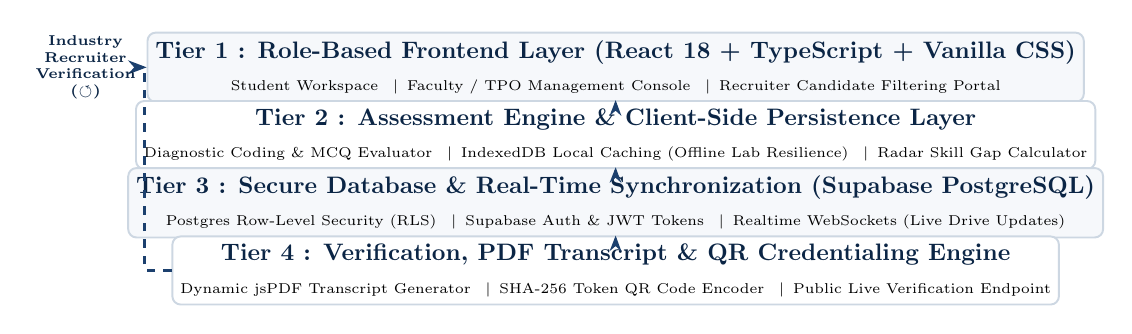
\begin{tikzpicture}[
      scale=0.86,every node/.style={transform shape},
      tierBox/.style={draw=BorderColor,fill=LightSilver,rounded corners=3pt,
                      minimum width=11.6cm,minimum height=0.74cm,
                      line width=0.7pt,align=center},
      arDown/.style={-{Stealth[scale=0.85]},thick,SlateBlue}
    ]

    % Tier 1: Role-Based Presentation Layer
    \node(t1)[tierBox] at (0, 1.95) {%
      \textbf{\color{Navy}Tier 1 : Role-Based Frontend Layer (React 18 + TypeScript + Vanilla CSS)}\\[1.5pt]
      \fontsize{6.2}{7.5}\selectfont
      Student Workspace \enspace\textbar\enspace
      Faculty / TPO Management Console \enspace\textbar\enspace
      Recruiter Candidate Filtering Portal};

    % Tier 2: Offline Persistence & Assessment Layer
    \node(t2)[tierBox,fill=white] at (0, 0.95) {%
      \textbf{\color{Navy}Tier 2 : Assessment Engine \& Client-Side Persistence Layer}\\[1.5pt]
      \fontsize{6.2}{7.5}\selectfont
      Diagnostic Coding \& MCQ Evaluator \enspace\textbar\enspace
      IndexedDB Local Caching (Offline Lab Resilience) \enspace\textbar\enspace
      Radar Skill Gap Calculator};

    % Tier 3: Database & Security Layer
    \node(t3)[tierBox] at (0, -0.05) {%
      \textbf{\color{Navy}Tier 3 : Secure Database \& Real-Time Synchronization (Supabase PostgreSQL)}\\[1.5pt]
      \fontsize{6.2}{7.5}\selectfont
      Postgres Row-Level Security (RLS) \enspace\textbar\enspace
      Supabase Auth \& JWT Tokens \enspace\textbar\enspace
      Realtime WebSockets (Live Drive Updates)};

    % Tier 4: Verification & Export Layer
    \node(t4)[tierBox,fill=white] at (0, -1.05) {%
      \textbf{\color{Navy}Tier 4 : Verification, PDF Transcript \& QR Credentialing Engine}\\[1.5pt]
      \fontsize{6.2}{7.5}\selectfont
      Dynamic jsPDF Transcript Generator \enspace\textbar\enspace
      SHA-256 Token QR Code Encoder \enspace\textbar\enspace
      Public Live Verification Endpoint};

    % Downward Data Flow Arrows
    \draw[arDown] (t1) -- (t2);
    \draw[arDown] (t2) -- (t3);
    \draw[arDown] (t3) -- (t4);

    % Left-Margin Feedback Arrow
    \draw[-{Stealth[scale=0.95]},dashed,SlateBlue,line width=0.9pt]
      (t4.west) -- ++(-0.40,0)
      |- node[pos=0.5,left,font=\fontsize{5.8}{7}\selectfont\bfseries,color=Navy,align=center]%
      {Industry\\Recruiter\\Verification\\($\circlearrowleft$)}
      (t1.west);
  \end{tikzpicture}

  \vspace{0.10cm}
  \begin{tcolorbox}[
    enhanced,colback=LightSilver,colframe=BorderColor,
    arc=2pt,boxrule=0.6pt,
    left=6pt,right=6pt,top=2.5pt,bottom=2.5pt]
    \centering\fontsize{6.5}{7.8}\selectfont
    \textbf{\color{Navy}Architecture Pipeline:}\enspace
    $\text{Student Assessment} \xrightarrow{\quad}
    \text{Offline IndexedDB Cache} \xrightarrow{\quad}
    \text{Supabase PostgreSQL \& RLS} \xrightarrow{\quad}
    \text{Drive Auto-Filter} \xrightarrow{\quad}
    \text{QR Verification} \circlearrowleft$
  \end{tcolorbox}
\end{frame}

% ------------------------------------------------------------
% SLIDE 9 — SYSTEM MODULES (Clean & Uniform)
% ------------------------------------------------------------
\begin{frame}[t]{System Modules}
  \begin{columns}[T]
    % Left Column: Modules 1 to 4
    \begin{column}{0.485\textwidth}
      \begin{tcolorbox}[modcard,title={1.\;Diagnostic Skill Assessment Module}]
        \fontsize{6.0}{7.0}\selectfont
        \begin{itemize}\setlength{\itemsep}{0pt}
          \item Domain-specific technical and coding challenges.
          \item Real-time skill radar charts mapping strengths and gaps.
        \end{itemize}
      \end{tcolorbox}\vspace{0.03cm}

      \begin{tcolorbox}[modcard,title={2.\;Faculty Milestone Verification Module}]
        \fontsize{6.0}{7.0}\selectfont
        \begin{itemize}\setlength{\itemsep}{0pt}
          \item Faculty review student lab projects and repositories.
          \item Awards authenticated digital badges to verified milestones.
        \end{itemize}
      \end{tcolorbox}\vspace{0.03cm}

      \begin{tcolorbox}[modcard,title={3.\;Placement \& Internship Drive Hub}]
        \fontsize{6.0}{7.0}\selectfont
        \begin{itemize}\setlength{\itemsep}{0pt}
          \item TPOs and companies post jobs with custom criteria.
          \item Automated candidate pre-filtering and Kanban pipelines.
        \end{itemize}
      \end{tcolorbox}\vspace{0.03cm}

      \begin{tcolorbox}[modcard,title={4.\;Offline-First IndexedDB Cache Layer}]
        \fontsize{6.0}{7.0}\selectfont
        \begin{itemize}\setlength{\itemsep}{0pt}
          \item Client-side persistence for test drafts and task logs.
          \item Prevents data loss during campus lab network failures.
        \end{itemize}
      \end{tcolorbox}
    \end{column}

    % Right Column: Modules 5 to 7 + Synthesis
    \begin{column}{0.485\textwidth}
      \begin{tcolorbox}[modcard,title={5.\;Institutional Skill Analytics (TPO Console)}]
        \fontsize{6.0}{7.0}\selectfont
        \begin{itemize}\setlength{\itemsep}{0pt}
          \item Batch-wide skill heatmaps across academic semesters.
          \item Early identification of weak student cohorts for training.
        \end{itemize}
      \end{tcolorbox}\vspace{0.03cm}

      \begin{tcolorbox}[modcard,title={6.\;Recruiter Candidate Screening Module}]
        \fontsize{6.0}{7.0}\selectfont
        \begin{itemize}\setlength{\itemsep}{0pt}
          \item Competency-based multi-parameter candidate filtering.
          \item Direct access to verified project repositories and scores.
        \end{itemize}
      \end{tcolorbox}\vspace{0.03cm}

      \begin{tcolorbox}[modcard,title={7.\;QR-Authenticated Transcript Generator}]
        \fontsize{6.0}{7.0}\selectfont
        \begin{itemize}\setlength{\itemsep}{0pt}
          \item Dynamic PDF generation using jsPDF and html2canvas.
          \item Tamper-proof QR code linking to live verification server.
        \end{itemize}
      \end{tcolorbox}\vspace{0.03cm}

      \begin{tcolorbox}[
        enhanced,colback=LightSilver,colframe=BorderColor,
        arc=2pt,boxrule=0.5pt,
        left=4pt,right=4pt,top=2pt,bottom=2pt]
        \centering\fontsize{6.0}{7.0}\selectfont\bfseries\color{Navy}
        All 7 modules operate as a synchronized, verified placement ecosystem.
      \end{tcolorbox}
    \end{column}
  \end{columns}
\end{frame}

% ------------------------------------------------------------
% SLIDE 10 — EXPECTED OUTCOME & DELIVERABLES
% ------------------------------------------------------------
\begin{frame}[t]{Project Status, Outcomes \& Deliverables}
  \begin{columns}[T]
    % Left Column: Outcome & Pilot Results
    \begin{column}{0.50\textwidth}
      \begin{navytitlecard}{Current Deployment \& Proven Results}
        \fontsize{6.8}{8.2}\selectfont
        \begin{itemize}\setlength{\itemsep}{1.2pt}
          \item \textbf{Active Department Pilot:}\;Live in department, used by students and faculty coordinators.
          \item \textbf{70\% Time Saved:}\;Eliminated manual TPO spreadsheet management and eligibility sorting.
          \item \textbf{100\% Data Integrity:}\;Replaced unverified Google Form claims with synchronized Postgres records.
        \end{itemize}
      \end{navytitlecard}

      \vspace{0.08cm}

      \begin{plaincard}{Validated Technical Metrics}
        \fontsize{6.8}{8.2}\selectfont
        \begin{itemize}\setlength{\itemsep}{1.2pt}
          \item \textbf{Zero Data Loss:}\;IndexedDB preserves test progress during lab network drops.
          \item \textbf{Instant QR Verification:}\;Sub-second validation of student scores during interviews.
        \end{itemize}
      \end{plaincard}
    \end{column}

    % Right Column: Deliverables & Alignment
    \begin{column}{0.48\textwidth}
      \begin{navytitlecard}{Key Completed Deliverables}
        \fontsize{6.8}{8.2}\selectfont
        \begin{enumerate}\setlength{\itemsep}{1pt}
          \item \textbf{Full Web Platform:}\;React 18 + TypeScript + Supabase.
          \item \textbf{Assessment Engine:}\;Automated diagnostic evaluation.
          \item \textbf{Role Dashboards:}\;Student, TPO, and Recruiter views.
          \item \textbf{PDF \& QR Transcripts:}\;Authenticated export generator.
        \end{enumerate}
      \end{navytitlecard}

      \vspace{0.08cm}

      \begin{tcolorbox}[
        enhanced,colback=LightSilver,colframe=BorderColor,
        arc=2pt,boxrule=0.7pt,
        left=5pt,right=5pt,top=2.5pt,bottom=2.5pt]
        \fontsize{6.5}{7.8}\selectfont\color{Charcoal}
        \textbf{\color{Navy}Institutional Value:}\;Provides an objective, verified academia-industry bridge turning self-declared resumes into \textbf{verifiable student competencies}.
      \end{tcolorbox}
    \end{column}
  \end{columns}

  \vspace{0.10cm}
  \begin{tcolorbox}[
    enhanced,colback=LightSilver,colframe=BorderColor,
    arc=2pt,boxrule=0.6pt,
    left=6pt,right=6pt,top=2.5pt,bottom=2.5pt]
    \centering\fontsize{6.5}{7.8}\selectfont
    \textbf{\color{Navy}Future Roadmap:}\;\textbf{1.} Automated Sandboxed Code Execution \enspace\textbullet\enspace \textbf{2.} AICTE/NCVET Skill Taxonomy Alignment \enspace\textbullet\enspace \textbf{3.} Multi-Department Campus Rollout.
  \end{tcolorbox}
\end{frame}

% ============================================================
\end{document}
